\subsection{Datasets}

The datasets on which the evaluations are done are retrieved from OpenML an online platform for machine learning research, which provides a database of machine learning datasets.

The datasets used for the evaluation follow the conditions show in Table \ref{table:conditions}.
\begin{table}[h]
\centering
\begin{tabular}{|c | c|  c|}
\hline
NumberOfInstances & > &  $5\cdot 10^5$\\
NumberOfInstances & < &  $10^7$ \\
NumberOfNumericFeatures & > & 5 \\
NumberOfNumericFeatures & < & 50 \\
NumberOfMissingValues & = & 0 \\
NumberOfSymbolicFeatures & = & 0 \\
\hline
\end{tabular}

\caption{Conditions for datasets used in the evaluation}
\label{table:conditions}
\end{table}

\subsection{Reduced number of Stages}
\label{section:evaluation_reduced_stages}
In this study, we are evaluating how Speculative K-Means can improve the performance of K-Means by reducing the number of stages required to reach convergence.

We conducted experiments on 10 datasets with the characteristics listed in Table \ref{table:conditions}, using both vanilla K-Means and Speculative K-Means with increasing number of clusters $k$ in the interval $[3,10]$. We measured the number of stages each algorithm took to reach convergence, which we defined as the point when the relative difference in inertia between two stages was below $10^{-3}$ or when the assignments are not changing anymore. Furthermore, we then calculated the ratio of the number of stages taken by Speculative K-Means to the number of stages taken by vanilla K-Means and plotted a histogram of these ratios. Additionally, we computed the ratio of the inertia of the final centroids obtained from the two algorithms.

In the experiments, we used a simple implementation of Speculative K-Means that utilized one thread for fast execution and one thread for slow execution. In this setup, we aimed to achieve most of the ratios below the value 0.5. This is because we were trying to reduce the execution time by more than what could be achieved through parallelization, which has the potential to reduce the overall execution time by up to 50\%. To achieve a 50\% reduction in overall time, it is therefore necessary to reduce the number of stages by at least half.

The results, shown in Figure \ref{fig:histogram_ratio_steps_inertia}, demonstrate that Speculative K-Means is often successful in reducing the number of stages to less than half the original amount in most cases, with most of the ratios in the range [0, 0.5]. Furthermore, the results show that the quality of the final centroids obtained using Speculative K-Means is not compromised, and may even be improved, despite the increased performance. This suggests that Speculative K-Means has the potential to significantly improve the efficiency of the K-Means algorithm without sacrificing solution quality.

\begin{figure}[h]
\centering
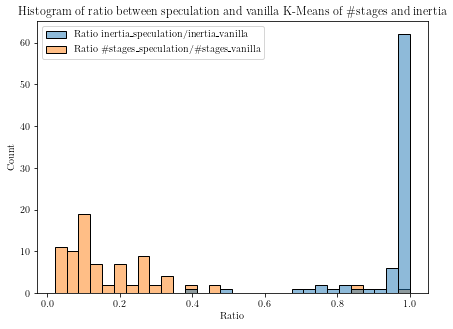
\includegraphics[width=\linewidth]{./plots/histogram_ratio_steps_inertia.png}
\caption{The histograms show the distribution of the ratio of the number of stages in speculative K-Means to the number of stages in vanilla K-Means (orange) and the ratio of the inertia in speculative K-Means to the inertia in vanilla K-Means (blue). The speculative execution used $subsample\_size=0.01$ and tracing \ref{section:final_stages} with $q=0.5$.}
\label{fig:histogram_ratio_steps_inertia}
\end{figure}

\subsection{Escaping local minima}
\label{section:evaluation_escaping_local_minima}
In this section, we show how Speculative K-Means can escape local minima through the use of the resampling centroid technique described in Section \ref{section:escaping_local_minima}. To demonstrate this, we conducted executions with increasing values of $k$ in $[3,10]$ on $10$ datasets with the characteristics shown in Table \ref{table:conditions}. We ran three versions of K-Means: vanilla K-Means,  K-Means++, and Speculative K-Means with centroid resampling. For all executions, we also computed the optimal solution and the respective inertia, and then calculated the ratio of the inertia of the solution found by each of the three methods to the optimal solution. Finally, we plotted histograms of these ratios for all three methods. In these executions, Vanilla and Speculative K-Means always started from the same initial centroids, whereas K-Means++ used its initialization technique. According to Figure \ref{fig:histogram_escape_local_minima}, it can be seen that Speculative K-Means had the highest number of instances where the ratio was close to 1, indicating that it was most successful in reaching the global minimum. Then it is followed by K-Means++, and finally by Vanilla K-Means.

These measurements suggest that Speculative K-Means, with centroid resampling, is indeed able to escape local minima without an initial time-cost, and in this particular case it also outperforms K-Means++.

\begin{figure}[h]
\centering
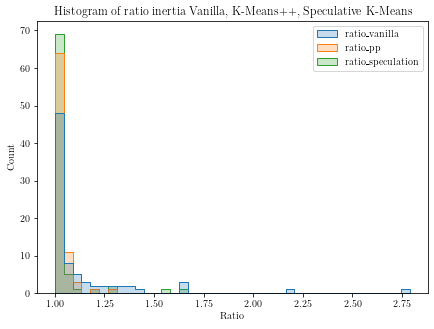
\includegraphics[width=\linewidth]{./plots/histogram_escape_local_minima.png}
\caption{The figure shows the ratio between the inertia of the centroids found by Vanilla, Speculative K-Means and K-Means++ to the optimal inertia. Speculative K-Means used a $subsample\_size=0.01$ and centroids resampling \ref{section:escaping_local_minima} with $p=0.5$}
\label{fig:histogram_escape_local_minima}
\end{figure}

\subsection{Overall time execution}

Previously, we demonstrated that the Speculation technique can significantly reduce the number of stages required for convergence in K-Means clustering. However, there are some time offsets to consider due to the repair and speculation processes, including the sampling of a subset of points for the fast execution and the repair step, which is the most time-consuming due to the computation of inertia of centroids from the fast and slow execution threads. This computation is similar in complexity to the Assignment step, which is the most time-consuming step in K-Means, as shown in Figure \ref{fig:ratio_k}.
In a simple implementation, there would be 1 Assignment step for the slow execution and 2 Inertia steps for the repair, totalling 3 steps with complexity comparable to the Assignment. This can be reduced to 2 steps by using the results from the computation of inertia in one stage to compute the Assignment step in the next stage.
As the Assignment step is the most time-consuming, each stage in Speculative K-Means requires approximately double the time of a stage in Vanilla K-Means at most. While halving the total number of stages can compensate for the increased time per stage, the overall time of execution would still be the same. Improving the computation of inertia through better parallelization or alternative approaches such as avoiding explicit computation of inertia could further improve the performance of Speculative K-Means. These possibilities could be explored in future work.
In Figure \ref{fig:histogram_time_execution}, we show the distribution of the ratios of number of stages and total time of execution between the execution of Speculative and Vanilla K-Means. Despite the drastic reduction in the number of stages, the total time of execution is not decreased the same way. A solution to the previously mentioned problem could potentially reduce the total time of execution to be more comparable to the reduced number of stages.

\begin{figure}[h]
\centering
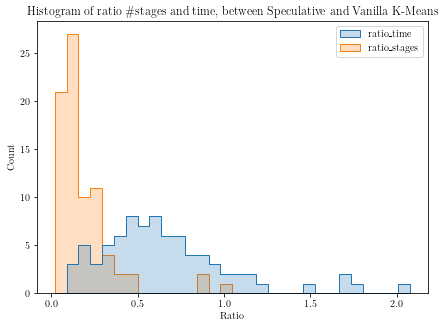
\includegraphics[width=\linewidth]{./plots/histogram_time_execution.png}
\caption{The figure shows the ratio between the \#stages and the total time of execution for convergence of Vanilla and Speculative K-Means. Speculative K-Means used a $subsample\_size=0.01$ and tracing with $q = 0.5$}
\label{fig:histogram_time_execution}
\end{figure}